% Chapter: Quantile, Robust and Constrained Reinforcement Learning
% Three formal equivalences between RL theory and decision theory:
% (1) distributional Bellman operators and risk measures,
% (2) constrained MDPs and shadow prices,
% (3) robust MDPs and ambiguity aversion.

The preceding chapters optimized expected returns. This chapter relaxes
that assumption in three directions: tracking full return distributions
rather than means (distributional RL), imposing constraints on secondary
objectives (constrained MDPs), and hedging against model misspecification
(robust MDPs).


%% ===================================================================
%% SECTION 1: DISTRIBUTIONAL RL AND RISK MEASURES
%% ===================================================================

\subsection{Distributional Reinforcement Learning and Risk Measures}
\label{subsec:distributional_rl}

Standard reinforcement learning characterizes a policy $\pi$ by the
expected return $V^\pi(s) = \mathbb{E}^\pi\bigl[\sum_{t=0}^\infty \gamma^t
R_t \mid S_0 = s\bigr]$. Distributional reinforcement learning instead
maintains the full random variable $Z^\pi(s,a) = \sum_{t=0}^\infty \gamma^t
R_t$ whose expectation is $Q^\pi(s,a)$. \citet{Bellemare2017} showed that
the Bellman equation has a distributional counterpart that propagates entire
distributions rather than expectations, and that this distributional operator
contracts in the Wasserstein metric.

Let $\mathcal{Z}$ denote the space of return-distribution functions mapping
state-action pairs to distributions over $\mathbb{R}$. The distributional
Bellman operator $\mathcal{T}^\pi$ is defined by
\begin{equation}
  \mathcal{T}^\pi Z(s,a) \stackrel{D}{=} R(s,a) + \gamma Z(S', A'),
  \quad S' \sim P(\cdot|s,a), \; A' \sim \pi(\cdot|S'),
  \label{eq:dist_bellman}
\end{equation}
where $\stackrel{D}{=}$ denotes equality in distribution.
\citet{Bellemare2017} proved that $\mathcal{T}^\pi$ is a $\gamma$-contraction
in the Wasserstein distance (informally, the minimum cost of reshaping one distribution into another) between distributions,
\begin{equation}
  \bar{d}_p(Z_1, Z_2) = \sup_{s,a} d_p\bigl(Z_1(s,a),\, Z_2(s,a)\bigr),
  \label{eq:wasserstein_metric}
\end{equation}
where $d_p$ is the $p$-Wasserstein distance between univariate
distributions. Since $\mathcal{T}^\pi$ is a contraction, iterating it
converges to a unique return distribution $Z^\pi$ under policy
$\pi$. For quantile representations, minimizing the quantile regression
loss~\eqref{eq:qrdqn_loss} is equivalent to minimizing the 1-Wasserstein
distance to the Bellman target \citep{Dabney2018a}, so QR-DQN and IQN
directly inherit this convergence guarantee.\footnote{$\mathcal{T}^\pi$
is not a contraction in total variation or KL divergence. The optimality operator $\mathcal{T}^*$ is not a contraction
in any distribution metric, though expected values still converge
\citep{Bellemare2017}.}

A standard DQN network outputs a single scalar $Q_\theta(s,a)$ per action
and minimizes the squared TD error
$(r + \gamma \max_{a'} Q_{\bar{\theta}}(s',a') - Q_\theta(s,a))^2$,
where $r$ is the observed reward, $s'$ is the next state, and
$\bar{\theta}$ denotes a slowly-updated target network.

\citet{Dabney2018a} introduced Quantile Regression DQN (QR-DQN), whose
network instead outputs $N$ values $\theta_1(s,a), \ldots, \theta_N(s,a)$
representing quantile locations of the return distribution, each with
equal probability $1/N$. The quantile regression loss for a single
quantile level $\tau \in (0,1)$ is
$\rho_\tau(u) = u(\tau - \mathbbm{1}\{u < 0\})$, which penalizes
underestimates by a factor of $\tau$ and overestimates by $1-\tau$.
The full QR-DQN loss sums this over all pairs of current quantiles $i$
and target quantiles $j$:
\begin{equation}
  L_{\text{QR}} = \frac{1}{N} \sum_{i=1}^{N} \sum_{j=1}^{N}
  \rho_{\hat{\tau}_i}\bigl(\underbrace{
    r + \gamma\, \theta_j^{\text{target}}(s', a^*)}_{\text{target quantile }j}
    - \underbrace{\theta_i(s,a)}_{\text{current quantile }i}
  \bigr),
  \label{eq:qrdqn_loss}
\end{equation}
where $\hat{\tau}_i = (2i-1)/(2N)$ is the midpoint of the $i$-th quantile
interval, $\theta_j^{\text{target}}$ comes from the target network, and
$a^* = \arg\max_{a'} \frac{1}{N}\sum_j \theta_j(s',a')$ is the greedy
action under the mean return.\footnote{The resulting projected operator is
a $\gamma$-contraction in the $\infty$-Wasserstein metric
\citep{Dabney2018a}.}

\citet{Dabney2018b} extended this to Implicit Quantile Networks (IQN).
Instead of outputting a fixed set of $N$ quantiles, the IQN network takes
a quantile level $\tau \in [0,1]$ as an additional input and outputs the
corresponding return value $F_{Z}^{-1}(\tau; s,a)$. The IQN loss has
the same pairwise structure, but with quantile levels sampled
continuously:
\begin{equation}
  L_{\text{IQN}} = \frac{1}{KK'} \sum_{i=1}^{K} \sum_{j=1}^{K'}
  \rho_{\tau_i}\bigl(
    r + \gamma\, F_{Z}^{-1}(\tau'_j; s', a^*)
    - F_{Z}^{-1}(\tau_i; s, a)
  \bigr),
  \label{eq:iqn_loss}
\end{equation}
where $\tau_1, \ldots, \tau_K$ and $\tau'_1, \ldots, \tau'_{K'}$ are
independent draws from $U([0,1])$, and $K, K'$ are the number of
samples per update. Because the quantile levels are sampled rather than
fixed, IQN learns the full continuous quantile function rather than a
discrete approximation. This continuous representation is the key bridge
to risk-sensitive control.

An agent that maximizes expected return is indifferent between a certain
payoff of 100 and a coin flip paying 0 or 200. In many applications this
is inadequate: a portfolio manager, a robot near a cliff, or a firm
facing bankruptcy all care about the shape of the return distribution, not
just its mean. Distributional RL provides the return distribution; what
remains is a principled way to convert that distribution into a scalar
objective that encodes the desired risk attitude. \citet{Yaari1987}
showed that this can be done with a distortion function
$h: [0,1] \to [0,1]$ (increasing, $h(0)=0$, $h(1)=1$) applied to the
cumulative distribution before integrating:
\begin{equation}
  \rho_h(Z) = \int_0^1 F_Z^{-1}(\tau) \, h'(1-\tau) \, d\tau.
  \label{eq:distortion_risk}
\end{equation}
This class includes the expected value ($h(\tau)=\tau$), Conditional
Value-at-Risk at level $\alpha$ ($h(\tau) = \min(\tau/\alpha, 1)$), and the
Cumulative Prospect Theory
\citep{TverskyKahneman1992}, which overweights tail outcomes relative to
their true probabilities. Since IQN can evaluate $F_Z^{-1}(\tau)$ at
any $\tau$, each of these risk measures reduces to choosing which quantiles
to average over and how to weight them. The network itself does not change;
only the sampling distribution of $\tau$ at decision time does. Sampling
$\tau$ from the non-uniform distribution $\beta(\tau) = h'(1-\tau)$ rather
than uniformly yields policies that maximize the distortion risk measure
$\rho_h$.

CVaR at level $\alpha$ (the expected return in the worst $\alpha$-fraction
of outcomes) is the most widely used case. In IQN, sampling
$\tau \sim U([0, \alpha])$ instead of $U([0,1])$ yields a CVaR-optimal
policy. CVaR can also be optimized exactly via dynamic programming on an
augmented state space \citep{Bauerle2011}, or through its equivalence to
robust MDPs with adversarial transition reweighting
\citep{Chow2015}.\footnote{Risk-averse dynamic programming requires the
risk measure to satisfy a recursive nestedness property (the
multi-period risk decomposes into nested single-period evaluations, as
the Bellman equation does for expected value)
\citep{Ruszczynski2010}. \citet{Hau2023} showed that popular decompositions
for CVaR are suboptimal regardless of discretization, correcting earlier
claims. \citet{Tamar2015} extended the policy gradient theorem to coherent
risk objectives as an alternative to the distributional approach.
\citet{Prashanth2016} proved consistency of CPT-value estimation from
sampled returns.}


\subsubsection{Simulation Study: Risk-Sensitive Inventory Management}
\label{subsec:sim_risk_inventory}

A newsvendor MDP with fat-tailed demand illustrates the mechanism.
The agent manages inventory over a 10-period horizon with state
$s \in \{0, \ldots, 15\}$ (current stock) and action $a \in \{0, \ldots, 5\}$
(order quantity). Demand follows a mixture distribution,
$D \sim 0.8 \cdot \text{Poisson}(3) + 0.2 \cdot \text{Poisson}(10)$,
creating occasional demand spikes that make risk preferences
matter.\footnote{Per-step reward:
$5 \cdot \min(s+a, D) - 2a - 1 \cdot (s+a-D)^+ - 8 \cdot (D-s-a)^+$.
The stockout penalty (8) exceeds the holding cost (1), so risk-averse
agents should carry more safety stock.}
A single IQN network is trained for 50{,}000 episodes with
$\tau \sim U([0,1])$, then evaluated under two $\tau$-sampling
distributions: $U([0,1])$ for risk-neutral and $U([0, 0.05])$ for
CVaR$_{95}$. Table~\ref{tab:risk_inventory} reports results over
50{,}000 evaluation episodes alongside the exact DP oracle.

\begin{table}[h]
\centering
\caption{Risk-sensitive inventory management. The CVaR$_{95}$ policy
sacrifices mean return for improved worst-case performance by ordering
more safety stock.}
\label{tab:risk_inventory}
\begin{tabular}{lcccc}
\hline
Policy & Mean Return & CVaR$_{95}$ & CVaR$_{99}$ & Avg.\ Order \\
\hline
DP Oracle & 40.4 & $-52.6$ & $-98.3$ & 2.56 \\
IQN-Neutral & 37.4 & $-57.8$ & $-104.0$ & 2.44 \\
IQN-CVaR$_{95}$ & 35.8 & $-55.0$ & $-97.5$ & 3.30 \\
\hline
\end{tabular}
\end{table}

The IQN-Neutral policy recovers 93\% of the DP oracle's mean return.
Switching to CVaR$_{95}$ at decision time trades 1.6 points of mean
return for 2.8 points of improved tail performance, achieved by
ordering more safety stock (3.30 versus 2.44 units per period).


%% ===================================================================
%% SECTION 2: CONSTRAINED MDPs
%% ===================================================================

\subsection{Constrained Markov Decision Processes}
\label{subsec:constrained_mdps}

Many decision problems involve optimizing a primary objective
subject to constraints on secondary costs. A firm maximizes profit subject
to a budget; a regulator maximizes welfare subject to safety thresholds; an
advertiser maximizes conversions subject to a spending limit. The theory of
constrained MDPs (CMDPs) provides a unified framework for these problems.

A constrained MDP augments the standard MDP
$(\mathcal{S}, \mathcal{A}, P, r, \gamma)$ with $K$ auxiliary cost
functions $c_k: \mathcal{S} \times \mathcal{A} \to \mathbb{R}$ and
constraint thresholds $q_k$. The agent maximizes the primary objective
subject to
\begin{equation}
  \max_\pi \; \mathbb{E}^\pi\Bigl[\sum_{t=0}^\infty \gamma^t r(S_t, A_t)\Bigr]
  \quad \text{subject to} \quad
  \mathbb{E}^\pi\Bigl[\sum_{t=0}^\infty \gamma^t c_k(S_t, A_t)\Bigr]
  \leq q_k, \quad k = 1, \ldots, K.
  \label{eq:cmdp}
\end{equation}

The key insight of \citet{Altman1999} is that this problem becomes a linear
program when reformulated over \emph{occupation measures} (the discounted fraction of
time spent in each state-action pair). The occupation measure of policy
$\pi$ is
\begin{equation}
  \nu^\pi(s,a) = (1-\gamma) \sum_{t=0}^\infty \gamma^t
  \mathbb{P}(S_t = s, A_t = a \mid \pi),
  \label{eq:occupation_measure}
\end{equation}
which satisfies the flow conservation constraints (probability flowing
into each state from transitions equals probability flowing out via
actions)
\begin{equation}
  \sum_a \nu(s,a) = (1-\gamma)\mu_0(s) + \gamma \sum_{s',a'} P(s|s',a')
  \nu(s',a') \quad \text{for all } s \in \mathcal{S}.
  \label{eq:bellman_flow}
\end{equation}
Since both the objective and
constraints are linear in $\nu$, and the feasible set forms a
polytope,\footnote{The feasible occupation measures form a bounded convex
set (polytope) defined by non-negativity, the Bellman flow conservation
equations, and the $K$ linear constraint inequalities.} the CMDP becomes a
standard LP. By Carath\'eodory's theorem,\footnote{Carath\'eodory's theorem
states that any point in the convex hull of a set in $\mathbb{R}^d$ can be
written as a convex combination of at most $d+1$ extreme points. The
unconstrained MDP polytope has deterministic policies as its vertices, and
the optimal LP solution sits at a vertex, which is why unconstrained optimal
policies are deterministic. Adding $K$ constraint inequalities introduces up
to $K$ additional dimensions along which the optimum may lie in the interior,
so the optimal solution is a convex combination of at most $K+1$ vertices.}
optimal CMDP policies mix at most $K+1$ deterministic policies for $K$
constraints.

The LP formulation yields \emph{strong duality} under Slater's
condition.\footnote{Slater's condition requires the existence of a feasible
policy $\pi'$ satisfying all constraints with strict inequality:
$\mathbb{E}^{\pi'}[\sum_t \gamma^t c_k(S_t,A_t)] < q_k$ for all $k$.}
The dual problem is
\begin{equation}
  \min_{\lambda \geq 0} \max_\pi \; L(\pi, \lambda)
  = \mathbb{E}^\pi\Bigl[\sum_{t=0}^\infty \gamma^t \bigl(
    r(S_t,A_t) - \sum_{k=1}^K \lambda_k c_k(S_t,A_t)
  \bigr)\Bigr] + \sum_{k=1}^K \lambda_k q_k,
  \label{eq:cmdp_lagrangian}
\end{equation}
and the optimal dual variable $\lambda_k^*$ is the \emph{shadow price} of
the $k$-th constraint. By the envelope theorem,
$\partial V^* / \partial q_k = \lambda_k^*$: the marginal change in optimal
value per unit relaxation of constraint $q_k$. This is the same shadow price
that appears in the linear programming dual of resource allocation
problems.

\citet{Paternain2019} extended this result beyond the LP formulation.
Despite the non-convexity of the objective in policy parameters, they proved
that constrained RL has \emph{zero duality gap}: the optimal dual value
equals the primal. The proof exploits the convexity of the occupancy measure
set and applies a minimax theorem. This means the CMDP can be solved
exactly via dual ascent on the Lagrange multipliers, even when using
parametric policy classes, with an approximation error bounded by the
expressiveness of the parametrization.


Zero duality gap means the CMDP can be solved by iterating between two
steps: for fixed multiplier $\lambda$, solve the unconstrained MDP with
reward $r(s,a) - \sum_k \lambda_k c_k(s,a)$; then update $\lambda$ by
gradient ascent on the dual~\eqref{eq:cmdp_lagrangian}.

\citet{Achiam2017} gave the foundational trust-region instantiation.
At iteration $k$, the policy update solves
\begin{equation}
  \max_\pi \; \mathbb{E}_{s \sim d^{\pi_k}\!, a \sim \pi}
    \bigl[A^r_{\pi_k}(s,a)\bigr]
  \quad \text{s.t.} \quad
  J_{C_i}(\pi_k) + \frac{1}{1-\gamma}
    \mathbb{E}_{s \sim d^{\pi_k}\!, a \sim \pi}
    \bigl[A^{C_i}_{\pi_k}(s,a)\bigr] \leq d_i,
  \quad
  \bar{D}_{\mathrm{KL}}(\pi \| \pi_k) \leq \delta,
  \label{eq:cpo_update}
\end{equation}
where $A^r_{\pi_k}$ and $A^{C_i}_{\pi_k}$ are the advantage functions for
the reward and the $i$-th cost, $d^{\pi_k}$ is the discounted state
visitation distribution, and
$\bar{D}_{\mathrm{KL}}(\pi\|\pi_k)
= \mathbb{E}_{s \sim \pi_k}[D_{\mathrm{KL}}(\pi(\cdot|s)\|\pi_k(\cdot|s))]$.
For the exact solution to~\eqref{eq:cpo_update}, monotone reward improvement
and per-iterate constraint satisfaction are
guaranteed.\footnote{\citet{Achiam2017} bound the worst-case constraint
degradation at
$O(\sqrt{\delta}\,\gamma\varepsilon/(1-\gamma)^2)$, where $\varepsilon$
bounds the cost advantage, via Pinsker's inequality. The implemented
Constrained Policy Optimization (CPO) algorithm solves a quadratic
approximation to~\eqref{eq:cpo_update}; the hard guarantee applies to the
exact solution.}\textsuperscript{,}\footnote{Subsequent theoretical work
sharpened convergence rates for primal-dual CMDP methods:
\citet{Tessler2019} proved almost-sure convergence of a three-timescale
actor-critic-multiplier scheme (RCPO) to a local Lagrangian optimum;
\citet{Ding2020} established the first non-asymptotic
$O(1/\sqrt{T})$ rate for both optimality gap and constraint violation
(dimension-free, via Fisher information geometry);
\citet{Liu2022cmdp} improved this to $O(\log(T)/T)$ using policy mirror
descent; and \citet{Ying2022} achieved $O(1/T)$ with entropy
regularization.}

In practice, the dominant method is PPO-Lagrangian, which replaces the
trust-region constraint in~\eqref{eq:cpo_update} with the PPO clipped
surrogate objective applied to the Lagrangian advantage
$\hat{A}^\lambda_t = \hat{A}^r_t - \lambda \hat{A}^c_t$:
\begin{equation}
  \max_\theta \; \mathbb{E}_{s,a \sim \pi_{\theta_k}}
  \Bigl[\min\bigl(
    \rho_t \hat{A}^\lambda_t,\;
    \mathrm{clip}(\rho_t, 1{-}\epsilon, 1{+}\epsilon)\,\hat{A}^\lambda_t
  \bigr)\Bigr],
  \qquad
  \rho_t = \frac{\pi_\theta(a_t|s_t)}{\pi_{\theta_k}(a_t|s_t)},
  \label{eq:ppo_lag_objective}
\end{equation}
where $\hat{A}^r_t$ and $\hat{A}^c_t$ are generalized advantage estimates
computed from two separate critics $V^r_\phi(s)$ and $V^c_\psi(s)$ via
$\hat{A}_t = \sum_{l=0}^{T-t}(\gamma\lambda_{\mathrm{GAE}})^l \delta_{t+l}$
with TD residuals
$\delta_t = r_t + \gamma V(s_{t+1}) - V(s_t)$ (analogously for cost).
After each policy update, the multiplier is adjusted by
projected gradient ascent on the constraint violation:
\begin{equation}
  \lambda_{t+1}
  = \bigl[\lambda_t + \eta\bigl(\hat{J}_C(\pi_\theta) - d\bigr)\bigr]_+.
  \label{eq:dual_update}
\end{equation}
\citet{Stooke2020} refined this update with a PID controller that dampens the multiplier oscillations characteristic of naive dual
ascent.\footnote{The FSRL library \citep{Liu2024fsrl} provides a
pip-installable implementation of PPO-Lagrangian alongside CPO and
TRPO-Lagrangian.}


\subsubsection{Simulation Study: Carbon-Constrained Production}
\label{subsec:sim_carbon_production}

A factory maximizes manufacturing profit subject to a carbon
emissions budget. The state is (inventory level, demand regime),
where inventory $\in \{0,\ldots,8\}$ and demand switches between
low and high regimes via a Markov chain. The action is
(production level, energy source), where production $\in \{0,1,2,3\}$
and energy is dirty (cheap, 3.0 tons CO$_2$ per unit) or clean
(expensive, 0.5 tons per unit). The reward is daily profit; the
cost is CO$_2$ emitted. The carbon budget $d$ is set to 30\% of the
unconstrained optimum's discounted emissions, and the LP dual
yields an analytical shadow price $\lambda^* = 1.20$.\footnote{The
constrained LP over occupation measures (18 states $\times$ 8
actions = 144 variables) is solved exactly with HiGHS. The shadow
price $\lambda^*$ is the dual variable on the carbon constraint,
interpretable as the Pigouvian tax that internalizes the emissions
externality.}
The CMDP is
\begin{equation}
  \max_\pi \; \mathbb{E}^\pi\Bigl[\sum_{t=0}^\infty \gamma^t
    \underbrace{\bigl(p \min(I_t + a^{\mathrm{prod}}_t,\, D_t)
    - \kappa_{e_t} a^{\mathrm{prod}}_t
    - h\,(I_t + a^{\mathrm{prod}}_t - D_t)^+\bigr)}_{r(S_t, A_t)}\Bigr]
  \quad \text{s.t.} \quad
  \mathbb{E}^\pi\Bigl[\sum_{t=0}^\infty \gamma^t
    \underbrace{\xi_{e_t}\, a^{\mathrm{prod}}_t}_{c(S_t, A_t)}\Bigr]
  \leq d,
  \label{eq:carbon_cmdp}
\end{equation}
where $p = 10$ is the unit price, $\kappa_e \in \{2, 5\}$ is the
production cost for dirty and clean energy respectively,
$h = 1$ is the holding cost, $\xi_e \in \{3.0, 0.5\}$ is the
emission rate, $D_t$ is stochastic demand, and $\gamma = 0.95$.

Table~\ref{tab:carbon_results} and
Figure~\ref{fig:carbon_convergence} compare three methods:
the constrained LP oracle, unconstrained Q-learning, and
Lagrangian Q-learning with dual ascent
on~\eqref{eq:dual_update}. Unconstrained Q-learning converges
near the DP optimum (return 255 versus 273) but violates the
carbon budget by a factor of three (cost 96 versus $d = 31$).
The learned multiplier rises from zero, overshoots to
$\lambda \approx 3.2$ before settling at $\lambda \approx 1.40$,
near the analytical shadow price $\lambda^* = 1.20$.
The overshoot is the characteristic oscillation of naive dual
ascent that \citet{Stooke2020}'s PID controller is designed
to dampen. Because the transient spike drives the policy
toward clean energy more aggressively than necessary, the
final cost (27) undershoots the budget (31), leaving the
Lagrangian agent slightly too conservative (return 180 versus
the LP optimum of 186). The LP optimal policy is stochastic,
mixing dirty and clean energy at a single state; Q-learning
recovers a deterministic approximation.

\begin{table}[h]
\centering
\caption{Carbon-constrained production results. Budget $d = 31.35$.}
\label{tab:carbon_results}
\begin{tabular}{lrrcc}
\hline
Method & Return & Cost & Budget & $\lambda$ \\
\hline
LP Oracle & 186.4 & 31.35 & Y & 1.20 \\
Unconstrained Q-learning & 257.8 $\pm$ 3.2 & 99.08 $\pm$ 2.62 & N & -- \\
Lagrangian Q-learning & 178.4 $\pm$ 4.0 & 28.44 $\pm$ 3.60 & Y & 1.40 $\pm$ 0.00 \\
\hline
\end{tabular}

\end{table}

\begin{figure}[h]
\centering
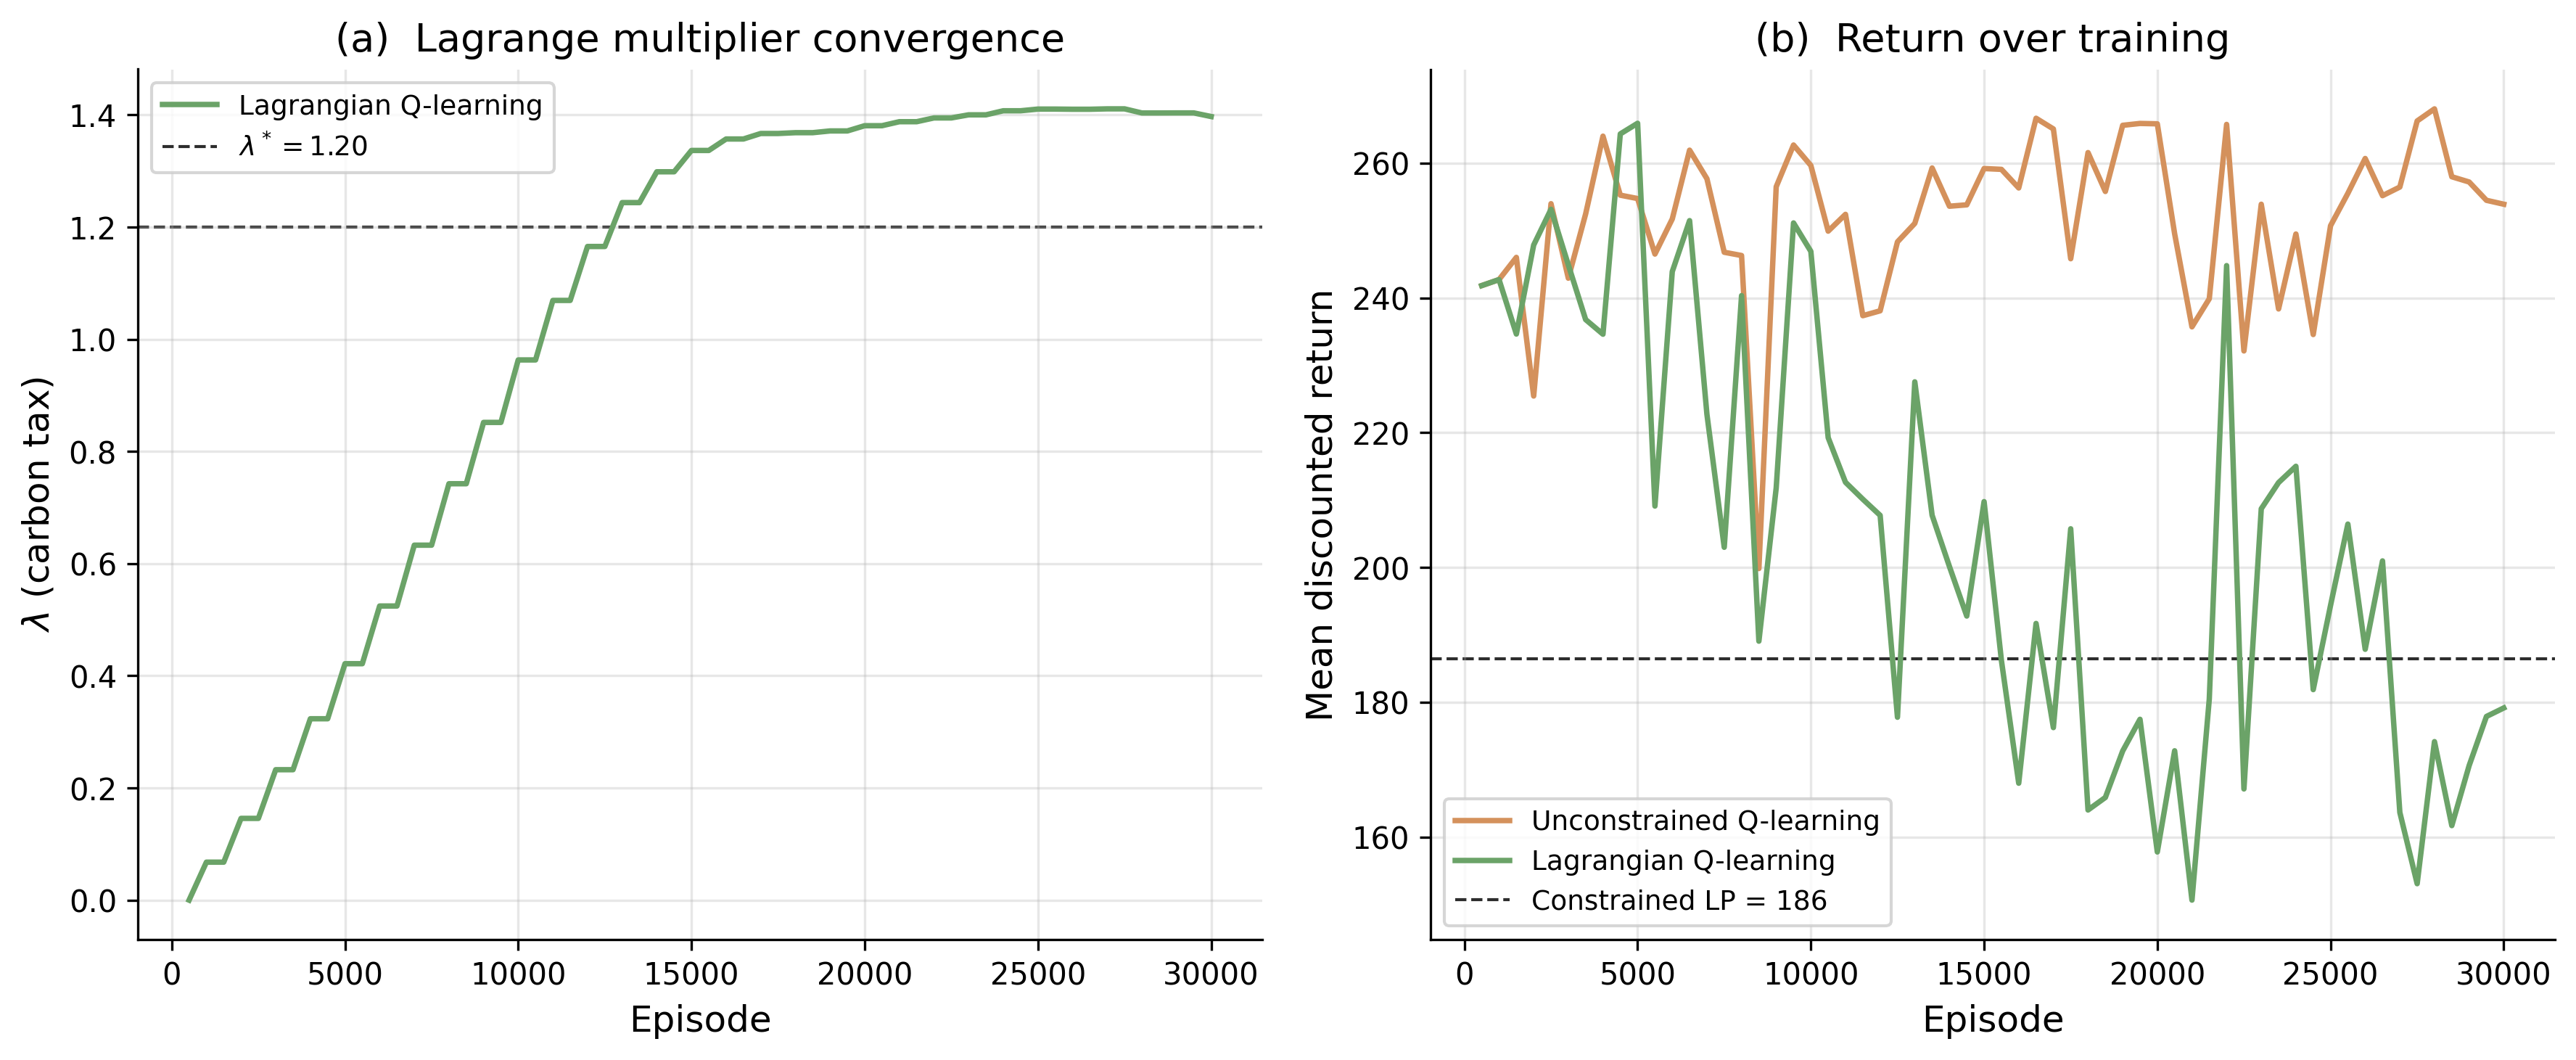
\includegraphics[width=\textwidth]{../ch11_dist_robust_constrained/sims/carbon_constrained_production_convergence.png}
\caption{(a) Lagrange multiplier $\lambda$ over training episodes,
with the LP shadow price $\lambda^*$ as the dashed reference.
(b) Mean discounted return for unconstrained and Lagrangian
Q-learning, with the constrained LP optimum as the dashed reference.}
\label{fig:carbon_convergence}
\end{figure}


%% ===================================================================
%% SECTION 3: ROBUST MDPs AND AMBIGUITY AVERSION
%% ===================================================================

\subsection{Robust MDPs and Ambiguity Aversion}
\label{subsec:robust_mdps}

When the transition kernel $P(s'|s,a)$ is known imprecisely, standard
dynamic programming may produce policies that perform well under the
nominal model\footnote{The nominal model $p_0(\cdot|s,a)$ is the agent's
best estimate of the transition kernel, typically estimated from data or
specified by a simulator.} but fail under plausible alternatives. Robust
MDPs address this by optimizing against worst-case transitions within an
uncertainty set around the nominal model.

\citet{Iyengar2005} defined the robust Bellman operator
\begin{equation}
  (TV)(s) = \max_a \min_{p \in \mathcal{P}(s,a)}
  \bigl\{r(s,a) + \gamma \, p \cdot V\bigr\},
  \label{eq:robust_bellman}
\end{equation}
where $\mathcal{P}(s,a)$ is an uncertainty set of transition
distributions for each state-action pair and $p_0(\cdot|s,a)$ is the
nominal transition kernel. Under the rectangularity assumption (the uncertainty sets are independent
across state-action pairs, so the joint set is a Cartesian product),
$T$ is a $\gamma$-contraction in
the sup-norm, so robust value iteration and policy iteration converge
with the same guarantees as their standard counterparts (recall
Section~\ref{section:rl_algorithms}); the only change is substituting $T$
for the standard Bellman operator.\footnote{Rectangularity means
$\mathcal{P} = \prod_{s,a} \mathcal{P}(s,a)$. Without it, the problem
becomes NP-hard \citep{Wiesemann2013}.} For
KL balls $\mathcal{P}(s,a) = \{p : \text{KL}(p \| p_0) \leq
\kappa\}$,\footnote{A KL ball of radius $\kappa$ around the nominal
contains all distributions ``close'' to $p_0$ in an information-theoretic
sense. For example, if $p_0 = (0.1, 0.3, 0.4, 0.2)$ across four states,
a ball with $\kappa = 0.1$ allows distributions like
$(0.15, 0.35, 0.35, 0.15)$ but not $(0.5, 0.5, 0, 0)$, which would be
too far from the nominal. \citet{Barillas2009} proposed calibrating
$\kappa$ (equivalently $\theta$) via detection error probabilities.
When KL sets are insufficient because $p_0$ assigns zero probability to
relevant outcomes, Wasserstein balls
$\{Q : W_p(Q, P_0) \leq \epsilon\}$ are the alternative
\citep{Esfahani2018, GrandClement2021, Yu2023}.} the inner minimization
has the closed-form solution
$q^*(s') \propto p_0(s'|s,a) \exp(-\gamma V(s')/\theta)$, an
exponential tilting of nominal transitions toward low-value states,
where $\theta$ is the Lagrange multiplier on the KL
constraint \citep{Nilim2005}.\footnote{\citet{HansenSargent2001}
independently derived the same operator from decision theory as
``multiplier preferences,'' in which the agent maximizes expected utility
penalized by the cost of distorting beliefs away from the reference model:
$\sup_c \inf_Q \{\mathbb{E}_Q[U(c)] + \theta \cdot
\text{KL}(Q\|P)\}$, where $\theta$ is the price of model uncertainty.
\citet{Petersen2000} proved that KL-robust MDPs, multiplier preferences,
and risk-sensitive control with exponential utility
$\mathbb{E}_P[\exp(-\text{cost}/\theta)]$ are three descriptions of the
same problem; see also \citet{Whittle1981}, \citet{Jacobson1973},
\citet{Fleming1992}.}\textsuperscript{,}\footnote{\citet{Maccheroni2006}
axiomatized variational preferences, in which the agent evaluates each
act under the worst-case belief penalized by a divergence cost:
$V(f) = \min_p \{\int u(f)\,dp + c(p)\}$, nesting maxmin EU
\citep{GilboaSchmeidler1989}, Hansen-Sargent, and mean-variance as
special cases. \citet{Strzalecki2011} showed KL is the unique penalty
satisfying a natural invariance axiom; \citet{HansenSargent2024}
provided a recent comprehensive treatment.}


\subsubsection{Algorithms for Robust RL}
\label{subsubsec:robust_algorithms}

The robust Bellman operator~\eqref{eq:robust_bellman} is a drop-in
replacement for the standard Bellman target. Robust Q-learning replaces
the TD target with its worst-case counterpart:
\begin{equation}
  Q(s,a) \leftarrow Q(s,a) + \alpha\Bigl[
    r + \gamma \min_{p \in \mathcal{P}(s,a)} \sum_{s'} p(s')
    \max_{a'} Q(s',a') - Q(s,a)
  \Bigr],
  \label{eq:robust_q_learning}
\end{equation}
where the inner minimization uses the exponential tilting for KL balls or
bisection for TV and chi-squared
sets.\footnote{Sample complexity for learning robust policies scales
polynomially in $|\mathcal{S}||\mathcal{A}|$: \citet{Panaganti2022}
established the first bounds under $(s,a)$-rectangular uncertainty for TV,
KL, and chi-squared sets; \citet{clavier2024robust} improved the rates for
model-based approaches.}

For high-dimensional problems where tabular methods and explicit
uncertainty sets are infeasible, \citet{Pinto2017} introduced Robust
Adversarial Reinforcement Learning (RARL):
\begin{equation}
  \max_{\pi_{\text{agent}}} \min_{\pi_{\text{adv}}} \;
  \mathbb{E}\Bigl[\sum_{t=0}^\infty \gamma^t
    r(s_t, a_t, a_t^{\text{adv}})
  \Bigr],
  \label{eq:rarl}
\end{equation}
where $a_t^{\text{adv}}$ is the adversary's action. Training alternates
between updating the agent policy $\pi_{\text{agent}}$ via TRPO or PPO
with the adversary fixed, then updating the adversary
$\pi_{\text{adv}}$ with the agent fixed. The adversary's action space is
problem-specific: joint torques for locomotion, force perturbations for
manipulation. The resulting agent policies are more conservative, with
wider stability margins; in locomotion tasks, robust agents adopt lower
center-of-gravity gaits. \citet{Pinto2017} demonstrated that policies
trained against an adversary in simulation transferred to physical robots
more reliably than standard PPO policies.

\citet{Derman2021} proved that entropy regularization provides implicit
robustness. The soft Bellman equation used in SAC,
\begin{equation}
  V(s) = \tau \log \sum_a \exp\bigl(Q(s,a)/\tau\bigr),
  \label{eq:soft_bellman}
\end{equation}
is equivalent to solving a robust MDP with reward uncertainty set
$\{r' : \text{KL}(r' \| r) \leq \kappa\}$, where the entropy temperature
$\tau$ maps directly to the robustness radius $\kappa$. Adding a
value-regularization term extends this to robustness against transition
misspecification.\footnote{The ``Twice Regularized MDP'' (R$^2$-MDP)
combines policy regularization (reward robustness) with value
regularization (transition robustness). Standard SAC training already
implements the reward-robust component; transition robustness requires an
additional penalty on the divergence between learned and nominal dynamics
models.} Standard SAC training therefore already implements reward-robust
RL; the robustness radius is controlled by $\tau$.

These three approaches offer different trade-offs. Robust Q-learning
requires an explicit uncertainty set but provides exact minimax guarantees
for tabular problems. RARL avoids specifying an uncertainty set by learning
the adversary, making it practical for continuous control, but provides no
formal robustness certificate. Entropy regularization provides implicit
robustness at zero additional implementation cost for practitioners already
using SAC, but ties the robustness radius to the temperature parameter.

\subsubsection{Simulation Study: Consumption-Savings Under Model Mismatch}
\label{subsec:sim_robust_consumption}

A consumption-savings agent with constant relative risk aversion (CRRA) utility
$u(c) = c^{1-\sigma}/(1-\sigma)$, $\sigma = 2$, receives stochastic
income $y \in \{1,\ldots,5\}$ each period and chooses how much to consume
versus save at gross return $R = 1.02$, with $\gamma = 0.95$. The robust
Bellman equation for this problem is
\begin{equation}
  V(w) = \max_{c \in \{0,\ldots,w\}} \Bigl\{
    u(c) + \gamma \min_{q:\,\text{KL}(q\|p_0) \leq \kappa}
    \sum_{y} q(y)\, V\bigl(R(w-c) + y\bigr)
  \Bigr\},
  \label{eq:robust_consumption}
\end{equation}
where $w$ is wealth, $c$ is consumption, and the inner minimization tilts
income probabilities toward low-income states via
$q^*(y) \propto p_0(y)\exp(-\gamma V(R(w-c)+y)/\theta)$. Seven policies
are computed: standard DP under the nominal income distribution
$p_0 = (0.05, 0.10, 0.20, 0.30, 0.35)$, robust DP at $\theta = 5$
(moderate) and $\theta = 2$ (high robustness), an oracle that knows the
true perturbed distribution
$\tilde{p} = (0.30, 0.30, 0.20, 0.10, 0.10)$, and three model-free
counterparts trained via tabular Q-learning under the nominal
model.\footnote{Standard Q-learning uses the usual TD target
$r + \gamma \max_{a'} Q(s',a')$; robust Q-learning replaces this with
the worst-case target~\eqref{eq:robust_q_learning}, using the nominal
kernel for the inner minimization (generative model setting).
Visit-count learning rates $\alpha = C/(C + N(s,a))$ with $C = 100$
and $\varepsilon$-greedy exploration decaying from 1.0 to 0.05 over
$10^5$ episodes.} All seven policies are then evaluated under both the
nominal and perturbed income models.

Table~\ref{tab:robust_consumption} reports discounted returns under both
models. Under the nominal model, all policies perform similarly.
Under the perturbed model, standard DP degrades by 76\% while the
$\theta = 2$ robust policy degrades by 72\%. The Q-learning and robust
Q-learning policies match their DP counterparts, confirming that the
model-free algorithms recover the same precautionary savings behavior.
Figure~\ref{fig:robust_consumption} shows the mechanism: robust agents
consume less at each wealth level, building a precautionary savings buffer
against adverse income realizations.

\begin{table}[h]
\centering
\caption{Discounted returns under nominal and perturbed income. DP policies
are computed via value iteration; Q-learning policies are trained under the
nominal model.}
\label{tab:robust_consumption}
\begin{tabular}{lrrr}
\hline
Method & Nominal & Perturbed & Degradation (\%) \\
\hline
Standard DP & $-4.941 \pm 0.001$ & $-8.694 \pm 0.004$ & $-76.0$ \\
Q-learning & $-4.941 \pm 0.001$ & $-8.692 \pm 0.005$ & $-75.9$ \\
Robust DP ($\theta$=5.0) & $-4.942 \pm 0.001$ & $-8.672 \pm 0.004$ & $-75.5$ \\
Robust Q-learning ($\theta$=5) & $-4.942 \pm 0.001$ & $-8.672 \pm 0.004$ & $-75.5$ \\
Robust DP ($\theta$=2.0) & $-4.948 \pm 0.001$ & $-8.486 \pm 0.004$ & $-71.5$ \\
Robust Q-learning ($\theta$=2) & $-4.948 \pm 0.001$ & $-8.486 \pm 0.004$ & $-71.5$ \\
Oracle & $-5.465 \pm 0.001$ & $-7.606 \pm 0.003$ & $-39.2$ \\
\hline
\end{tabular}
\end{table}

\begin{figure}[h]
\centering
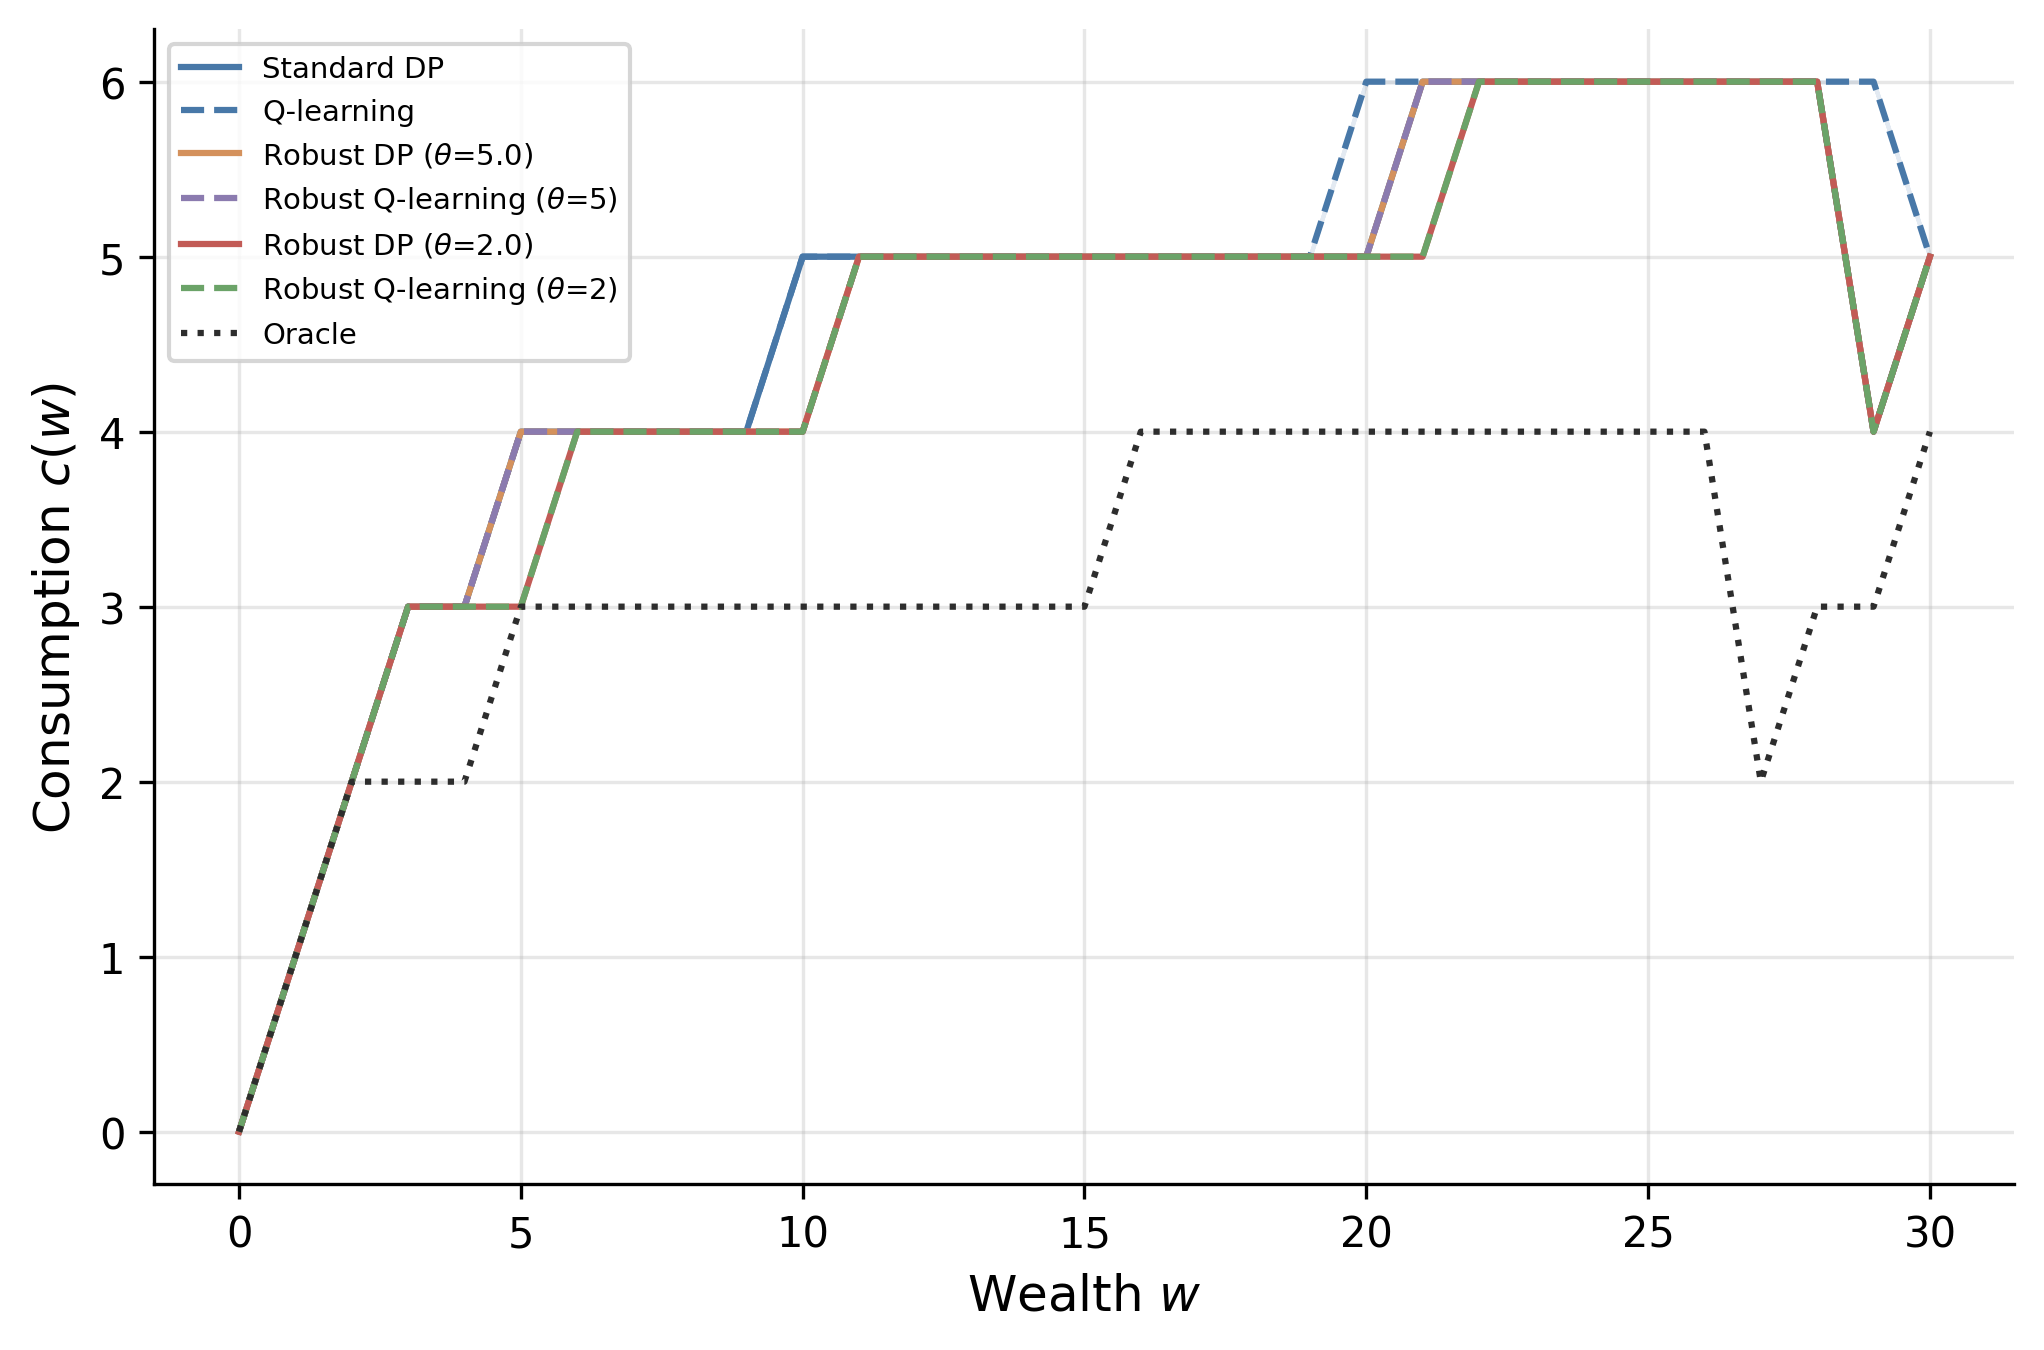
\includegraphics[width=0.85\textwidth]{../ch11_dist_robust_constrained/sims/robust_consumption_savings_policy.png}
\caption{Consumption policy $c(w)$ for each method. Dashed lines show
Q-learning policies; solid lines show DP. Robust agents consume less (save
more) than the nominal-model optimum.}
\label{fig:robust_consumption}
\end{figure}
